\section{Visualization}
\nblink{brats/13\_testnet\_hausdorff\_masks.ipynb}
\nblink{brats/14\_brats\_hausdorff\_masks.ipynb}

To visualize all the distances from the output of the masked image, a new blank image with the same size as the input image is generated. Next, we iterate over all the positions where masks have been
applied to input images. Each position has an associated Hausdorff distance which represents the distance of the output segment generated by the masked image and the ground truth segment.
At each position, we draw a circle with the same diameter as used when generating the mask. The color used to fill this circle represents the Hausdorff distance between the output segment generated by placing a circle at this exact position and the ground truth segment. The color map is scaled to the minimum and maximum Hausdorff distance encountered on all positions.

Figure \ref{hdm_visualization_sample} shows a masked input image (a), (b) shows the baseline output segment from the unchanged image and (c) shows the segment generated by the masked image.
The segment looks completely different from the ground truth, the calculated Hausdorff distance is therefore much bigger than the the distance between the unchanged output segment and the ground truth.

\begin{figure}[H]
    \centering
    \begin{subfigure}{.33\textwidth}
        \centering
        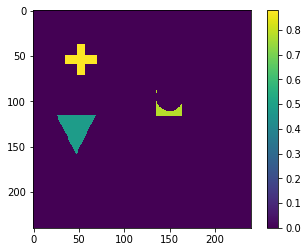
\includegraphics[width=\linewidth]{chapters/06_hdm/visualization/masked.png}
        \caption{Masked input image}
    \end{subfigure}%
    \begin{subfigure}{.33\textwidth}
        \centering
        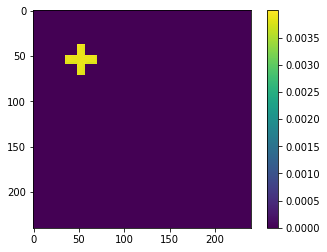
\includegraphics[width=\linewidth]{chapters/06_hdm/visualization/ground_truth.png}
        \caption{Ground truth segment}
    \end{subfigure}
        \begin{subfigure}{.33\textwidth}
        \centering
        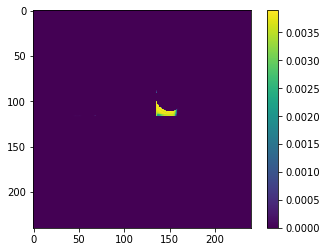
\includegraphics[width=\linewidth]{chapters/06_hdm/visualization/segment.png}
        \caption{Output segment from the masked image}
    \end{subfigure}
    \caption{The output segment (c) from the masked image (a) looks very different than the output segment from the unchanged image (b).}
    \label{hdm_visualization_sample}
\end{figure}

In Figure \ref{hdm_visualization_raw} we see a visualization of all the calculate Hausdorff distances. The dark circle on the upper right corner of the square corresponds to the masked circle from the masked image seen in Figure \ref{hdm_visualization_sample}. The circle is dark because the Hausdorff distance between the output segment (image (c)) and the ground truth (image (b)) is very big. The input image is processed by the canny edge detector and projected on top of the visualization.

To make the visualization interpretable, the original input image should be visible together with the visualization. Do avoid the distortion of the circle colors by projecting
the input image on top of the visualization, we apply the canny edge detector \cite{canny1987computational} on the input image before projecting it on top of the visualization.

\begin{figure}[H]
    \centering
    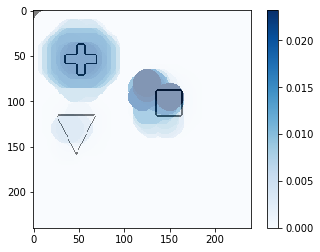
\includegraphics[width=8cm]{chapters/06_hdm/visualization/hdm_raw.png}
    \caption{Visualization of all Hausdorff distances corresponding to a mask at the same position. Intensity of the circle color is based on the Hausdorff distance at this position. The input image was processed with the canny edge detector.}
    \label{hdm_visualization_raw}
\end{figure}

Two things can happen when applying a mask (i.e. drawing a black circle) on an input image and running it through the network: The output segment is worse than the unchanged image or the output segment is actually better than from the unchanged segment. To differentiate these two cases, we split up the visualization generated above (Figure \ref{hdm_visualization_raw}). First, we calculate the baseline Hausdorff distance, i.e. the distance between the ground truth and the output segment generated by our network when feeding it with an unchanged input image. For the case where we are only interested in masks that decrease the accuracy of the output, we set all distances to zero which are smaller than the baseline distance (left image in Figure \ref{hdm_visualization_better_worsebetter}) and then subtract the baseline distance from all remaining distances. This way the diagram starts at zero. For the inverse case (right image in Figure \ref{hdm_visualization_better_worsebetter}), we set all distances to zero which are bigger than the baseline distance.

\begin{figure}[H]
    \centering
    \begin{subfigure}{.48\textwidth}
        \centering
        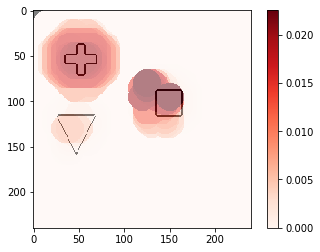
\includegraphics[width=\linewidth]{chapters/06_hdm/visualization/hdm_worse.png}
        \caption{Visualization of all masks which decrease the accuracy of the output segment when applied to an image}
    \end{subfigure}\hfill%
    \begin{subfigure}{.48\textwidth}
        \centering
        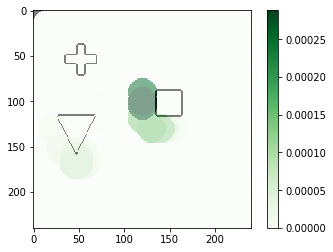
\includegraphics[width=\linewidth]{chapters/06_hdm/visualization/hdm_better.png}
        \caption{Visualization of all masks which increase the accuracy of the output segment when applied to an image}
    \end{subfigure}
    \caption{Visualization of regions in an image which decrease (left image) the segmentation output accuracy or increase (right image) it when occluded by a circle.}
    \label{hdm_visualization_better_worsebetter}
\end{figure}
